\documentclass[12pt,a4paper]{article}

\usepackage[utf8]{inputenc}
\usepackage[T1]{fontenc}
\usepackage[spanish]{babel}
\usepackage{lmodern}
\usepackage{geometry}
\usepackage{graphicx}
\usepackage{amsmath,amssymb}
\usepackage{array,booktabs,longtable}
\usepackage{float}
\usepackage{tikz}
\usetikzlibrary{babel,positioning}
\usepackage{microtype}
\usepackage{csquotes}
\usepackage{hyperref}
\usepackage[backend=biber,style=ieee]{biblatex}

\geometry{margin=2.5cm}
\graphicspath{{./}{../}}
\addbibresource{informe/referencias.bib}

\title{Comunicación distribuida mediante sockets TCP y gRPC}
\author{Jordan Loor \and Washington Apunte \and César Macías}
\date{Noviembre de 2026}

\begin{document}
\sloppy
\pagenumbering{roman}
\maketitle
\begin{center}
\textbf{Código de actividad:} GA-SUM-02\\
\textbf{Repositorio:} \texttt{github.com/jloors13/GA-SUM-02-gRPC-Sockets-TCP}
\end{center}
\tableofcontents
\clearpage
\pagenumbering{arabic}

\section{Comunicación TCP entre tres nodos}
\label{sec:tcp-jordan}

\subsection{Objetivo e hipótesis}

El objetivo fue implementar el intercambio de mensajes entre tres nodos por
sockets TCP y medir su latencia, throughput y comportamiento ante tres
solicitudes simultáneas. Como hipótesis previa, se esperaba que los relojes de
Lamport conservaran el orden causal de cada solicitud y su respuesta, y que
las mediciones variaran entre tamaños de mensaje bajo las mismas condiciones
locales. La dirección de esa variación no se presupuso.

La implementación TCP organiza la comunicación entre tres nodos, denominados
\texttt{nodo-A}, \texttt{nodo-B} y \texttt{nodo-C}. En la configuración
experimental, los tres se ejecutan en un mismo equipo y escuchan en la
dirección \texttt{127.0.0.1}, mediante los puertos 5000, 5001 y 5002,
respectivamente. Cada nodo puede iniciar solicitudes y atender las de los
otros. Esta disposición permite examinar el intercambio entre procesos sin
introducir las condiciones de una red entre equipos físicos.

\subsection{Arquitectura e intercambio de mensajes}

\begin{figure}[htbp]
\centering
\begin{tikzpicture}[>=stealth]
\node[draw,rounded corners,align=center] (a) at (0,0) {nodo-A\\127.0.0.1:5000};
\node[draw,rounded corners,align=center] (b) at (6,0) {nodo-B\\127.0.0.1:5001};
\node[draw,rounded corners,align=center] (c) at (3,-2.5) {nodo-C\\127.0.0.1:5002};
\draw[->] (a) -- node[above]{TCP/JSON} (b);
\draw[->] (b) -- node[right]{TCP/JSON} (c);
\draw[->] (c) -- node[below left]{TCP/JSON} (a);
\end{tikzpicture}
\caption{Rutas de comunicación entre los tres nodos del experimento.}
\label{fig:arquitectura-tcp}
\end{figure}

El cliente establece una conexión con el puerto del nodo de destino mediante
un socket TCP. La solicitud se codifica en UTF-8 como una línea JSON con los
campos \texttt{sender}, \texttt{timestamp} y \texttt{message}. El servidor lee
esa línea, valida el emisor, el timestamp y el mensaje, y devuelve otra línea
JSON. En una respuesta válida se incluyen el nodo que respondió, el instante
lógico de recepción, el instante lógico de envío de la respuesta y un acuse
\texttt{ACK}. El servidor utiliza un manejador de solicitudes por conexión,
lo que permite atender comunicaciones simultáneas.

Cada nodo mantiene un reloj lógico de Lamport. Antes de enviar, incrementa su
contador y adjunta el nuevo valor a la solicitud. El receptor actualiza su
reloj al máximo entre su valor local y el recibido, más una unidad; antes de
responder vuelve a incrementarlo. Al recibir la respuesta, el cliente
actualiza también su reloj. Así, los cuatro instantes de un intercambio
válido siguen el orden envío del cliente, recepción del servidor, envío de la
respuesta y recepción del cliente. Los eventos de envío y recepción se
registran en archivos CSV por nodo con el tipo de evento, el valor lógico y
la hora real. El archivo \texttt{data/tcp\_exchanges.csv} conserva además
los cuatro timestamps de cada intercambio experimental.

Los registros TCP muestran, por ejemplo, un evento \texttt{receive} del
\texttt{nodo-A} con valor lógico 4 y un evento \texttt{send} del
\texttt{nodo-B} también con valor 4. La igualdad de valores entre nodos es
posible: el reloj de Lamport ordena eventos causales, pero un valor igual no
demuestra simultaneidad física ni basta por sí solo para establecer una
relación causal entre esos dos eventos.

\subsection{Procedimiento experimental}

Se realizaron 20 intercambios entre los nodos A y B, B y C, y C y A, en ese
orden de envío. Para medir la latencia de
solicitud y respuesta se emplearon mensajes de 100 y 10.240 bytes. Cada
tamaño tuvo una fase de calentamiento, seguida de cinco repeticiones de cien
mediciones; las muestras de calentamiento no forman parte del resumen. El
throughput de cada repetición se calculó como cien mensajes divididos por la
duración de ese lote. También se lanzaron tres solicitudes concurrentes, una
por cada ruta, mediante tres hilos sincronizados al inicio.

Las mediciones se guardaron en el archivo \texttt{tcp\_latency.csv} y las tres
observaciones concurrentes en \texttt{tcp\_concurrency.csv}, ambos dentro de
\texttt{data/}. El módulo \texttt{tcp\_statistics.py}, ubicado en
\texttt{analysis/}, agrupó las latencias por tamaño de
mensaje y calculó media, mediana, mínimo, máximo, desviación estándar
muestral, percentil 95 (P95) y promedio de los valores de throughput
registrados. El resumen se encuentra en \texttt{tcp\_statistics.csv} dentro
de \texttt{data/}.

\subsection{Resultados de TCP}

La Tabla~\ref{tab:tcp-jordan-estadisticas} presenta las métricas obtenidas
de las 500 muestras de cada tamaño. Todos los tiempos están expresados en
milisegundos; el throughput corresponde al promedio de la columna de
mensajes por segundo de los lotes experimentales.

\begin{table}[htbp]
\centering
\caption{Resumen estadístico de la latencia y el throughput TCP}
\label{tab:tcp-jordan-estadisticas}
\begin{tabular}{lrr}
\hline
\textbf{Métrica} & \textbf{100 bytes} & \textbf{10.240 bytes} \\
\hline
Muestras & 500 & 500 \\
Media (ms) & 7,220525 & 4,850986 \\
Mediana (ms) & 6,322050 & 4,079050 \\
Mínimo (ms) & 2,764400 & 2,937700 \\
Máximo (ms) & 31,517900 & 29,215500 \\
Desviación estándar (ms) & 3,797761 & 3,491191 \\
P95 (ms) & 13,501700 & 7,165695 \\
Throughput promedio (mensajes/s) & 144,301253 & 204,265171 \\
\hline
\end{tabular}
\end{table}

En esta ejecución, los mensajes de 10.240 bytes tuvieron una latencia media
menor que los de 100 bytes. La diferencia describe las mediciones obtenidas
en el equipo local y no establece por sí sola una relación general entre el
tamaño del mensaje y el rendimiento de TCP. Los máximos, superiores a las
respectivas medias, muestran además que hubo observaciones más lentas dentro
de ambas series.

La prueba concurrente produjo las tres latencias de la
Tabla~\ref{tab:tcp-jordan-concurrencia}. Estas cifras describen una única
ejecución con tres solicitudes simultáneas y no constituyen una medición
exhaustiva de escalabilidad.

\begin{table}[htbp]
\centering
\caption{Latencias registradas en la prueba concurrente TCP}
\label{tab:tcp-jordan-concurrencia}
\begin{tabular}{llr}
\hline
\textbf{Emisor} & \textbf{Destino} & \textbf{Latencia (ms)} \\
\hline
\texttt{nodo-A} & \texttt{nodo-B} & 6,1154 \\
\texttt{nodo-B} & \texttt{nodo-C} & 6,2118 \\
\texttt{nodo-C} & \texttt{nodo-A} & 6,6787 \\
\hline
\end{tabular}
\end{table}

Las pruebas se efectuaron sobre la interfaz local. Por ello, las latencias
incluyen el procesamiento y la comunicación entre procesos del mismo equipo,
pero no representan retardos de una red física entre computadoras.

\section{El contrato \texttt{.proto} y Protocol Buffers}

Protocol Buffers es un formato para definir y serializar datos estructurados
que se usa junto con gRPC~\cite{niswar2024}
para que dos procesos intercambien mensajes sabiendo de antemano qué campos
existen y de qué tipo es cada uno. A diferencia del JSON de texto que usa
nuestra implementación TCP, donde la estructura no está escrita en ningún
archivo y el servidor accede a cada clave a mano, en Protocol Buffers la
estructura y los tipos se declaran en un archivo \texttt{.proto} y los mensajes
viajan en binario. Esto no elimina la validación de los valores: nuestro
servidor gRPC sigue rechazando el emisor vacío y el \texttt{timestamp}
negativo. Otra diferencia es el tratamiento de los campos ausentes: en
\texttt{proto3} un campo que no se envía llega con su valor por defecto
(cadena vacía o 0), mientras que en TCP la clave faltante provoca un
\texttt{KeyError} que el servidor detecta y responde como error. Además, gRPC
transporta estos mensajes sobre HTTP/2~\cite{rfc9113}, que a su vez funciona
sobre TCP~\cite{rfc9293}.

\subsection{El archivo \texttt{servicio.proto}}

El archivo \texttt{proto/servicio.proto} es el contrato entre el servidor y el
cliente gRPC: describe qué mensajes existen y qué función se puede llamar de
forma remota. Su contenido, sin comentarios, es el siguiente:

\begin{verbatim}
syntax = "proto3";

package mensajeria;

service ComunicacionNodos {
  rpc EnviarMensaje(Mensaje) returns (Acuse);
}

message Mensaje {
  string sender = 1;
  int64 timestamp = 2;
  string message = 3;
}

message Acuse {
  string sender = 1;
  int64 received_timestamp = 2;
  int64 timestamp = 3;
  string message = 4;
}
\end{verbatim}

Cada parte cumple una función:

\begin{itemize}
  \item \texttt{syntax = "proto3"} indica la versión del lenguaje de
        Protocol Buffers.
  \item \texttt{package mensajeria} agrupa las definiciones y evita choques
        de nombres con otros archivos.
  \item \texttt{service ComunicacionNodos} declara la función remota
        \texttt{EnviarMensaje}: recibe un \texttt{Mensaje} y devuelve un
        \texttt{Acuse}.
  \item \texttt{Mensaje} es lo que envía el cliente y equivale al JSON
        \texttt{\{sender, timestamp, message\}} de TCP.
  \item \texttt{Acuse} es lo que responde el servidor y equivale a la
        respuesta JSON de TCP.
  \item Los números \texttt{= 1}, \texttt{= 2}, \dots{} identifican cada campo
        dentro del mensaje binario. En el binario no viajan los nombres de los
        campos, solo estos números.
\end{itemize}

\subsection{Tamaño del mensaje: Protocol Buffers frente a JSON}

Para comparar el tamaño se codificó el mismo mensaje de prueba
(\texttt{sender="nodo-A"}, \texttt{timestamp=5}, \texttt{message="hola"}) en
las dos formas. En nuestro mensaje de prueba, Protocol Buffers ocupa 16 bytes
y el JSON generado con \texttt{json.dumps} ocupa 55 bytes. Estas cifras
corresponden solo al contenido del mensaje, sin contar las cabeceras de gRPC ni
de TCP, y no se pueden generalizar a otros mensajes: con textos largos, la
diferencia relativa será menor, porque el contenido del texto ocupa lo mismo
en ambos formatos.

Otros trabajos han comparado gRPC con REST. En uno, gRPC obtuvo mejor
rendimiento en transferencias de datos grandes, pero la diferencia no resultó
estadísticamente significativa~\cite{ain2025}; en otro, las aplicaciones con
gRPC fueron, en general, más eficientes y escalables, aunque consumieron más
CPU~\cite{jcsi2024}. Sobre la serialización, se ha señalado que reducir el
tamaño del mensaje influye más en la latencia de extremo a extremo que la
velocidad de serialización~\cite{maltsev2024}. Nuestra comparación solo mide
el tamaño en bytes, no la latencia.

\subsection{Elección del tipo \texttt{int64}}

Los tres campos de tiempo guardan el valor del reloj de Lamport. Aunque este
reloj nunca es negativo y \texttt{uint64} también sería válido, se eligió
\texttt{int64} por dos razones. Primero, facilita la compatibilidad con
lenguajes sin enteros sin signo nativos, como Java, si en el futuro se escribe
un cliente en otro lenguaje. Segundo, con \texttt{int64} el servidor puede
recibir un valor negativo y rechazarlo de forma controlada con
\texttt{INVALID\_ARGUMENT}, como comprueba la prueba
\texttt{test\_timestamp\_negativo}. En Python ambos tipos se leen como
\texttt{int}, así que la elección no cambia el resto del código del servidor.

\subsection{Generación del código}

El archivo \texttt{.proto} no se ejecuta. Se procesa con
\texttt{grpc\_tools.protoc} desde la raíz del repositorio:

\begin{verbatim}
python -m grpc_tools.protoc -I. \
    --python_out=. --grpc_python_out=. \
    proto/servicio.proto
\end{verbatim}

Este comando genera dos archivos:

\begin{itemize}
  \item \texttt{servicio\_pb2.py}: las clases \texttt{Mensaje} y
        \texttt{Acuse} para crear y leer mensajes.
  \item \texttt{servicio\_pb2\_grpc.py}: la clase base
        \texttt{ComunicacionNodosServicer}, de la que hereda nuestro servidor,
        y el \texttt{ComunicacionNodosStub}, que usa el cliente para llamar a
        \texttt{EnviarMensaje} como si fuera una función local.
\end{itemize}

La opción \texttt{-I.} toma la raíz del repositorio como punto de partida, de
modo que el import generado queda como \texttt{from proto import servicio\_pb2}.
\section{Servidor gRPC}

El servidor gRPC es el componente de cada nodo que recibe los mensajes de los
demás nodos. Implementa la única función remota que declara el contrato,
\texttt{EnviarMensaje(Mensaje) returns (Acuse)}, y cumple el mismo papel que
\texttt{tcp\_server.py} en la implementación TCP: recibe un mensaje, actualiza
el reloj de Lamport, registra los eventos y responde con una confirmación. El
código está en \texttt{src/grpc/grpc\_server.py}, y cada nodo
(\texttt{nodo-A}, \texttt{nodo-B} y \texttt{nodo-C}) se inicia con su propia
dirección y puerto.

\subsection{Estructura del servidor}

La clase \texttt{ComunicacionNodosServicer} hereda de
\texttt{servicio\_pb2\_grpc.ComunicacionNodosServicer}, la clase base generada
a partir del \texttt{service} del archivo \texttt{.proto}. Su constructor
recibe tres datos y los guarda: el nombre del nodo (\texttt{node\_name}), su
reloj de Lamport (\texttt{clock}) y su registrador de eventos (\texttt{logger}).
Al recibirlos desde fuera, la clase no depende de cómo se crean, y la misma
lógica se puede reutilizar para los tres nodos.

La función \texttt{create\_server} arma el servidor: crea un
\texttt{grpc.server} con un \texttt{ThreadPoolExecutor} de 10 hilos
(\texttt{max\_workers=10}), registra el \emph{servicer} con
\texttt{add\_ComunicacionNodosServicer\_to\_server} y abre el puerto con
\texttt{add\_insecure\_port}. El \texttt{ThreadPoolExecutor} es lo que permite
atender varias llamadas a la vez: cada llamada que llega se ejecuta en un hilo
del grupo, de modo que, mientras una se procesa, otra puede empezar sin esperar
a que la primera termine, hasta un máximo de 10 simultáneas.

Esto marca una diferencia con la versión TCP. \texttt{TCPNodeServer} hereda de
\texttt{ThreadingTCPServer}, que crea un hilo nuevo por cada conexión sin
ningún límite, mientras que el servidor gRPC usa un grupo fijo de 10 hilos. El
grupo acota el número de hilos y, por tanto, el consumo de recursos, pero si
llegan más de 10 llamadas a la vez, las demás esperan a que se libere un
hilo.

\begin{figure}[htbp]
  \centering
  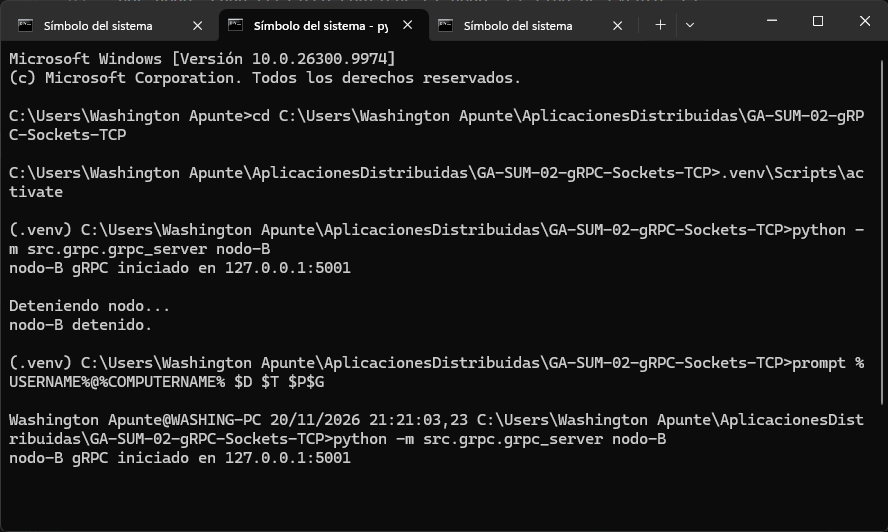
\includegraphics[width=\linewidth]{informe/capturas/captura_servidor.png}
  \caption{Inicio de un nodo del servidor gRPC.}
  \label{fig:servidor}
\end{figure}

\subsection{Qué hace \texttt{EnviarMensaje}}

Cada llamada ejecuta los siguientes pasos, en este orden:

\begin{enumerate}
  \item Validar la solicitud: se comprueba que el emisor no esté vacío y que
        el \texttt{timestamp} no sea negativo. Si algo falla, se rechaza la
        llamada y no se ejecuta ningún paso más.
  \item Llamar a \texttt{clock.after\_receive(request.timestamp)} para
        actualizar el reloj con el valor recibido, y registrar el evento
        \texttt{receive} con el valor que devuelve.
  \item Llamar a \texttt{clock.before\_send()} para incrementar el reloj antes
        de responder, y registrar el evento \texttt{send} con ese valor.
  \item Devolver un \texttt{Acuse} con el nombre del nodo como
        \texttt{sender}, el valor del paso 2 en \texttt{received\_timestamp},
        el valor del paso 3 en \texttt{timestamp} y el mensaje
        \texttt{"ACK: "} seguido del texto recibido.
\end{enumerate}

\begin{figure}[htbp]
  \centering
  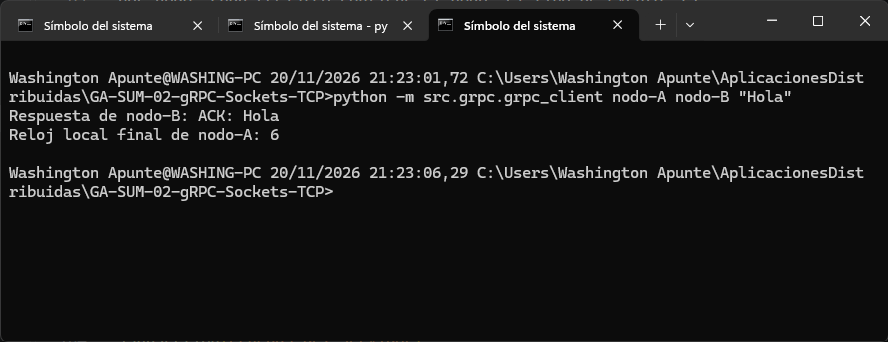
\includegraphics[width=\linewidth]{informe/capturas/captura_cliente.png}
  \caption{El cliente envía un mensaje y recibe el acuse del servidor.}
  \label{fig:cliente}
\end{figure}

\subsection{Validación y errores}

El servidor rechaza dos casos: un emisor vacío, con el mensaje
\texttt{"Emisor invalido"}, y un \texttt{timestamp} negativo, con el mensaje
\texttt{"Timestamp invalido"}. En ambos usa
\texttt{context.abort(grpc.StatusCode.INVALID\_ARGUMENT, \dots)}, que
interrumpe la función, de modo que no hace falta un \texttt{return}. En
\texttt{proto3} un campo \texttt{string} que no se envía llega como cadena
vacía, por lo que la misma comprobación cubre el emisor vacío y el emisor
ausente.

Los tipos de los campos ya los garantiza el contrato, por eso no se repiten
las comprobaciones de tipo que sí hace \texttt{tcp\_server.py}
(\texttt{isinstance} para \texttt{sender} y \texttt{message}, y
\texttt{type(timestamp) is not int} para el \texttt{timestamp}; esta última
forma también rechaza los valores booleanos). Del lado del cliente, la llamada rechazada se manifiesta
como una excepción \texttt{grpc.RpcError} con el código
\texttt{INVALID\_ARGUMENT} y el texto del error. Es el equivalente a la
respuesta \texttt{\{"error": \dots\}} de la versión TCP. Como la validación
ocurre antes de tocar el reloj, una solicitud rechazada no modifica el reloj
ni deja eventos registrados.

\begin{figure}[htbp]
  \centering
  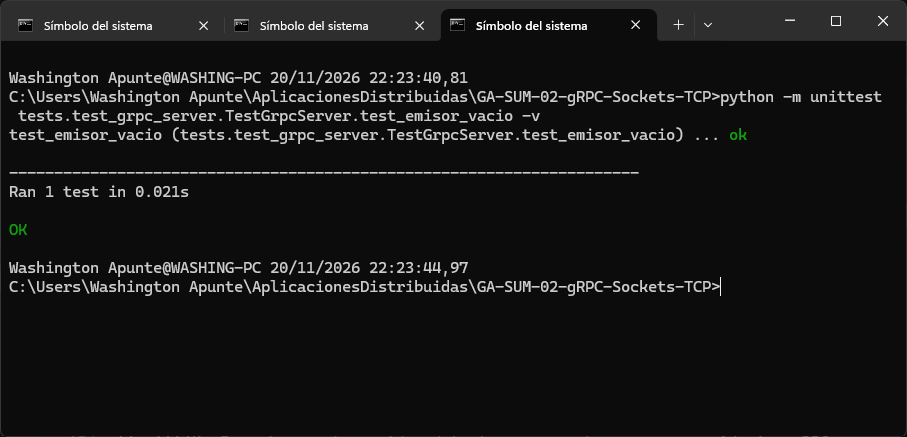
\includegraphics[width=\linewidth]{informe/capturas/captura_emisor_vacio.png}
  \caption{Prueba \texttt{test\_emisor\_vacio}: el servidor rechaza un emisor vacío.}
  \label{fig:vacio}
\end{figure}

\begin{figure}[htbp]
  \centering
  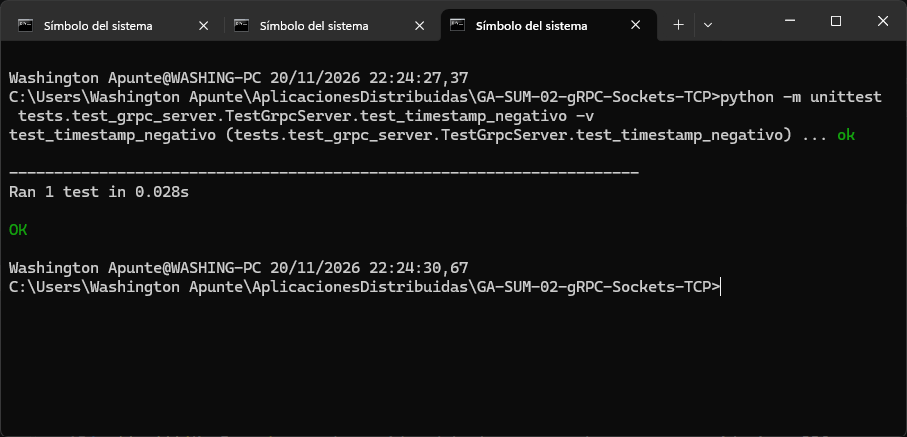
\includegraphics[width=\linewidth]{informe/capturas/captura_timestamp_negativo.png}
  \caption{Prueba \texttt{test\_timestamp\_negativo}: el servidor rechaza un \texttt{timestamp} negativo.}
  \label{fig:negativo}
\end{figure}

\subsection{Reloj de Lamport y registro de eventos}

El reloj de Lamport~\cite{lamport1978} se actualiza en dos puntos de \texttt{EnviarMensaje}:
\texttt{after\_receive} al recibir, que tiene en cuenta el \texttt{timestamp}
del emisor, y \texttt{before\_send} antes de responder. Por cada llamada
aceptada, el servidor registra dos eventos con \texttt{logger.log\_event}: uno
de tipo \texttt{receive} y otro de tipo \texttt{send}, ambos con el nombre del
nodo y el valor del reloj en ese momento.

Los eventos se escriben en \texttt{data/grpc\_events\_\textless{}nodo\textgreater{}.csv}, un archivo
por nodo. Cada registro contiene el nodo, el tipo de evento, el
\texttt{timestamp} de Lamport y la fecha y hora reales, igual que en la
implementación TCP, lo que permite comparar los dos mecanismos con el mismo
formato de datos.

Como el servidor atiende varias llamadas a la vez, el acceso concurrente al
reloj y al archivo es importante. Cada operación del reloj
(\texttt{time}, \texttt{before\_send} y \texttt{after\_receive}) está protegida
con un \texttt{Lock}, por lo que dos hilos no pueden obtener el mismo valor, y
el registrador de eventos usa otro \texttt{Lock} al escribir en el archivo. Sin
embargo, \texttt{EnviarMensaje} completo no es atómico: dos llamadas
simultáneas pueden intercalar sus pasos, de modo que los eventos de ambas
pueden aparecer mezclados en el CSV, aunque cada valor del reloj sigue siendo
único.

\begin{figure}[htbp]
  \centering
  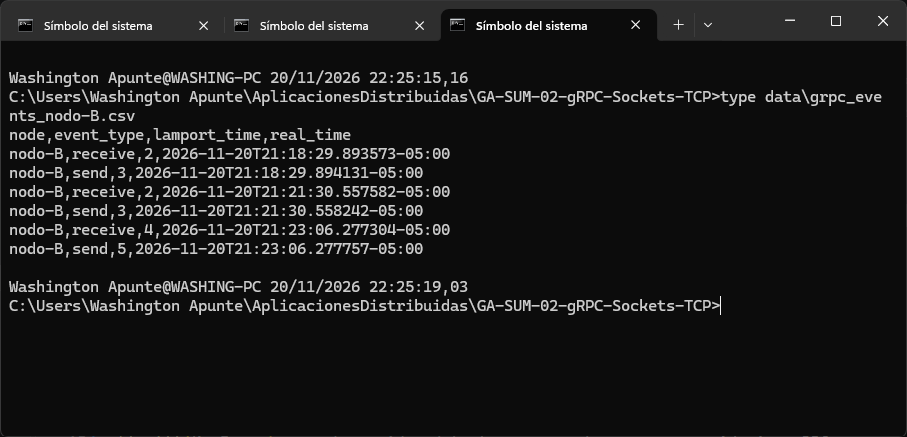
\includegraphics[width=\linewidth]{informe/capturas/captura_csv_eventos.png}
  \caption{Eventos \texttt{receive} y \texttt{send} registrados por \texttt{nodo-B}.}
  \label{fig:csv}
\end{figure}

\subsection{Pruebas del servidor}

Las pruebas del servidor están en \texttt{tests/test\_grpc\_server.py} y se
ejecutan con:

\begin{verbatim}
python -m unittest tests.test_grpc_server -v
\end{verbatim}

El archivo contiene 6 pruebas:

\begin{itemize}
  \item \texttt{test\_timestamp\_negativo}: comprueba que el servidor rechaza
        un \texttt{timestamp} negativo con \texttt{INVALID\_ARGUMENT} y que no
        se registra ningún evento.
  \item \texttt{test\_llamada\_valida}: envía un mensaje con \texttt{timestamp=5}
        y comprueba que la respuesta trae el nombre del nodo, el valor de
        reloj 6 al recibir, el valor 7 al responder y el texto
        \texttt{"ACK: hola"}.
  \item \texttt{test\_emisor\_vacio}: envía un mensaje con el emisor vacío y
        comprueba que se rechaza con \texttt{INVALID\_ARGUMENT} y que no se
        registra ningún evento.
  \item \texttt{test\_reloj\_crece\_entre\_llamadas}: hace dos llamadas seguidas y
        comprueba que el valor \texttt{received\_timestamp} de la segunda
        respuesta es mayor que el valor \texttt{timestamp} de la primera.
  \item \texttt{test\_registra\_receive\_y\_send}: hace una llamada con
        \texttt{timestamp=5} y comprueba que el registrador guarda exactamente
        2 eventos: \texttt{receive} con valor 6 y \texttt{send} con valor 7.
  \item \texttt{test\_concurrencia}: prueba de concurrencia. Se lanzaron 30 llamadas desde 10 hilos y no se repitió ningún
        \texttt{timestamp}. Esto demuestra que
        los valores del reloj no se repiten, no que las llamadas sean
        atómicas.
\end{itemize}

\begin{figure}[htbp]
  \centering
  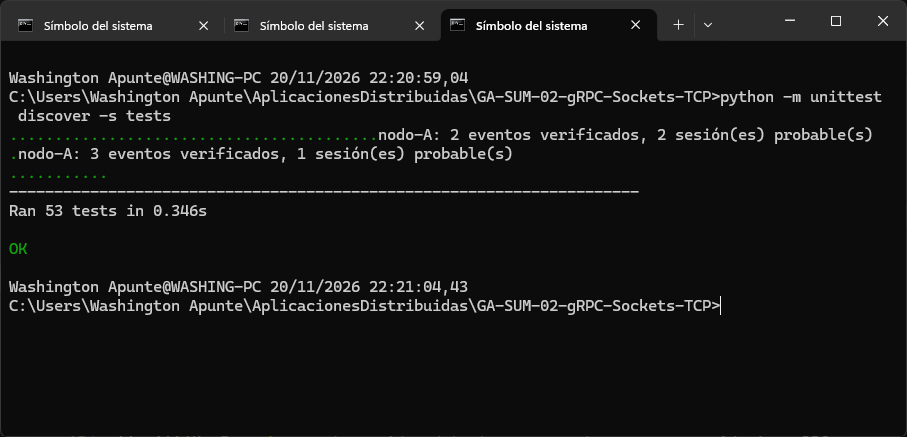
\includegraphics[width=\linewidth]{informe/capturas/captura_53_pruebas.png}
  \caption{Ejecución de las pruebas con \texttt{unittest}: todas pasan.}
  \label{fig:pruebas}
\end{figure}
\section{Cliente gRPC y ejecución experimental}

El cliente gRPC es el componente encargado de iniciar las comunicaciones hacia
los demás nodos distribuidos, coordinar los relojes lógicos de Lamport en el
origen y destino, y gestionar el ciclo de vida de las llamadas a través de
canales HTTP/2~\cite{rfc9113}. Su implementación reside en el módulo
\texttt{src/grpc/grpc\_client.py}, mientras que la automatización de las
pruebas de rendimiento y concurrencia se encuentra en
\texttt{src/grpc/grpc\_experiment.py}.

\subsection{Estructura e implementación del cliente}

El cliente implementa la función \texttt{send\_message}, cuyos parámetros
principales son la dirección (\texttt{host}), el puerto (\texttt{port}), el
nodo emisor (\texttt{sender}), la instancia local del reloj
(\texttt{clock}), el registrador de eventos (\texttt{logger}), el cuerpo del
mensaje (\texttt{message}) y un tiempo límite opcional (\texttt{timeout=5.0}).

A diferencia de la implementación basada en sockets TCP (\texttt{tcp\_client.py}),
donde se realiza manualmente la conexión del socket, la serialización JSON en
cadena de texto y la lectura por bloques con delimitadores, en gRPC se crea un
canal de comunicación mediante \texttt{grpc.insecure\_channel(f"\{host\}:\{port\}")}
y se instancia un \emph{stub} generado automáticamente:
\texttt{servicio\_pb2\_grpc.ComunicacionNodosStub(channel)}.

El envío se ejecuta a través del método síncrono:
\begin{verbatim}
response = stub.EnviarMensaje(request, timeout=timeout)
\end{verbatim}
donde \texttt{request} es un objeto fuertemente tipado de clase
\texttt{servicio\_pb2.Mensaje}. El uso del contexto \texttt{with} garantiza
el cierre controlado del canal al concluir la llamada o en caso de error.

\subsection{Gestión del reloj de Lamport y registro de eventos}

El algoritmo de Lamport~\cite{lamport1978} se sincroniza estrictamente en dos
instantes dentro de la función \texttt{send\_message}:

\begin{enumerate}
  \item \textbf{Antes de la transmisión:} Se invoca \texttt{clock.before\_send()},
        lo cual incrementa en una unidad el contador del reloj local. De inmediato
        se registra el evento de salida con
        \texttt{logger.log\_event(sender, "send", send\_timestamp)} y se asigna dicho
        valor al campo \texttt{timestamp} del mensaje gRPC.
  \item \textbf{Al recibir el acuse:} Tras la respuesta remota del servidor, se
        recupera el \texttt{response.timestamp} y se ejecuta
        \texttt{clock.after\_receive(response.timestamp)}. Esta función calcula
        $\max(C_{\text{local}}, C_{\text{remoto}}) + 1$, preservando la relación
        causal fundamental $a \to b \implies C(a) < C(b)$. Acto seguido se registra
        el evento \texttt{receive} en el archivo CSV del emisor.
\end{enumerate}

Ambos eventos se persisten en \texttt{data/grpc\_events\_\textless{}nodo\textgreater{}.csv},
asegurando paridad estructural con los registros de la arquitectura TCP.

\subsection{Manejo de excepciones y tolerancia a fallos}

El cliente envuelve la llamada gRPC en un bloque \texttt{try \dots\ except grpc.RpcError}.
Si el nodo destino se encuentra apagado, inalcanzable o rechaza la petición por
validación (por ejemplo, emisor vacío o \texttt{timestamp} negativo con
\texttt{StatusCode.INVALID\_ARGUMENT}), se captura la excepción nativa y se
transforma en un \texttt{RuntimeError} informativo:

\begin{verbatim}
except grpc.RpcError as error:
    raise RuntimeError(
        f"Error gRPC al enviar de {sender} a {host}:{port}: "
        f"{error.code().name} - {error.details()}"
    ) from error
\end{verbatim}

Esta abstracción previene bloqueos indefinidos del proceso y facilita el
diagnóstico de errores tanto en pruebas unitarias como en ejecuciones por
lotes.

\subsection{Entorno experimental de las corridas}

Para asegurar la reproducibilidad de las mediciones de latencia, rendimiento y
concurrencia, las ejecuciones experimentales de gRPC se llevaron a cabo bajo las
siguientes especificaciones:

\begin{itemize}
  \item \textbf{Hardware y plataforma:} Arquitectura x86\_64 (AMD64) con 16 núcleos
        lógicos de procesamiento, 16~GB de memoria RAM y sistema operativo
        Microsoft Windows 11.
  \item \textbf{Entorno de software:} Intérprete Python (versión 3.14 / 3.12),
        con las dependencias del proyecto instaladas desde \texttt{requirements.txt}:
        \texttt{grpcio}, \texttt{grpcio-tools}, \texttt{protobuf}, \texttt{pandas},
        \texttt{numpy} y \texttt{matplotlib}.
  \item \textbf{Nodos como procesos independientes en \texttt{localhost}:} Los tres
        nodos (\texttt{nodo-A}, \texttt{nodo-B} y \texttt{nodo-C}) se ejecutaron en
        el host local (\texttt{127.0.0.1}) en los puertos 5000, 5001 y 5002
        respectivamente. Cada nodo opera como un proceso/hilo aislado con su propio
        estado de memoria, su propio reloj lógico y su propio descriptor de archivo de
        eventos. La ejecución sobre el \emph{loopback} local elimina el sesgo de
        fluctuaciones externas de red (como latencias variables de Wi-Fi o congestión en
        enrutadores), permitiendo aislar el costo computacional intrínseco del protocolo
        y de la serialización Protocol Buffers frente a JSON~\cite{maltsev2024}.
\end{itemize}

\subsection{Automatización experimental (\texttt{grpc\_experiment.py})}

El script \texttt{src/grpc/grpc\_experiment.py} orquesta la batería completa de
pruebas de forma homogénea con los experimentos de TCP:

\begin{enumerate}
  \item \textbf{Intercambios deterministas en anillo:} 20 comunicaciones secuenciales
        siguiendo la topología \texttt{nodo-A} $\to$ \texttt{nodo-B} $\to$
        \texttt{nodo-C} $\to$ \texttt{nodo-A}, almacenando cada paso en
        \texttt{data/grpc\_exchanges.csv} para verificar la monotonía causal.
  \item \textbf{Medición de latencia por tamaño de carga útil:} Se evalúan mensajes
        cortos (100~bytes) y largos (10.240~bytes = 10~KB). Por cada tamaño se
        descartan las primeras muestras para eliminar el costo de arranque
        (\emph{warm-up}) y se registran 5 repeticiones de 100 muestras válidas,
        acumulando 1.000 mediciones almacenadas en \texttt{data/grpc\_latency.csv}.
  \item \textbf{Prueba de concurrencia:} Se lanzan tres solicitudes simultáneas hacia
        distintos nodos mediante \texttt{ThreadPoolExecutor}, registrando los tiempos
        en \texttt{data/grpc\_concurrency.csv} y validando que no se generen
        colisiones de estado en los servidores receptores.
\end{enumerate}

\subsection{Pruebas unitarias del cliente}

En el archivo \texttt{tests/test\_grpc\_client.py} se desarrollaron tres pruebas
automatizadas con el marco \texttt{unittest}:

\begin{itemize}
  \item \texttt{test\_envio\_valido\_y\_reloj\_lamport}: Verifica que un mensaje
        emitido por \texttt{nodo-A} hacia \texttt{nodo-B} retorne el acuse esperado
        (\texttt{"ACK: Mensaje de prueba"}), y que los cuatro timestamps cumplan
        estrictamente el orden causal ascendente:
        $t_{\text{recv}} > 1$, $t_{\text{ack}} > t_{\text{recv}}$ y
        $t_{\text{cliente final}} > t_{\text{ack}}$.
  \item \texttt{test\_error\_emisor\_vacio}: Comprueba que al enviar una cadena vacía
        como emisor, el cliente capture la respuesta del servidor y dispare
        satisfactoriamente una excepción \texttt{RuntimeError}.
  \item \texttt{test\_error\_servidor\_inaccesible}: Comprueba el comportamiento ante
        un puerto cerrado (5099) con un \texttt{timeout=1.0}, validando que el
        cliente lance \texttt{RuntimeError} sin quedar bloqueado indefinidamente.
\end{itemize}

Las tres pruebas se ejecutan con:
\begin{verbatim}
python -m unittest tests.test_grpc_client -v
\end{verbatim}
obteniendo resultado favorable (\texttt{OK}) en 1.7 segundos y consolidando un
total de 56 pruebas superadas en el repositorio.

\begin{figure}[htbp]
  \centering
  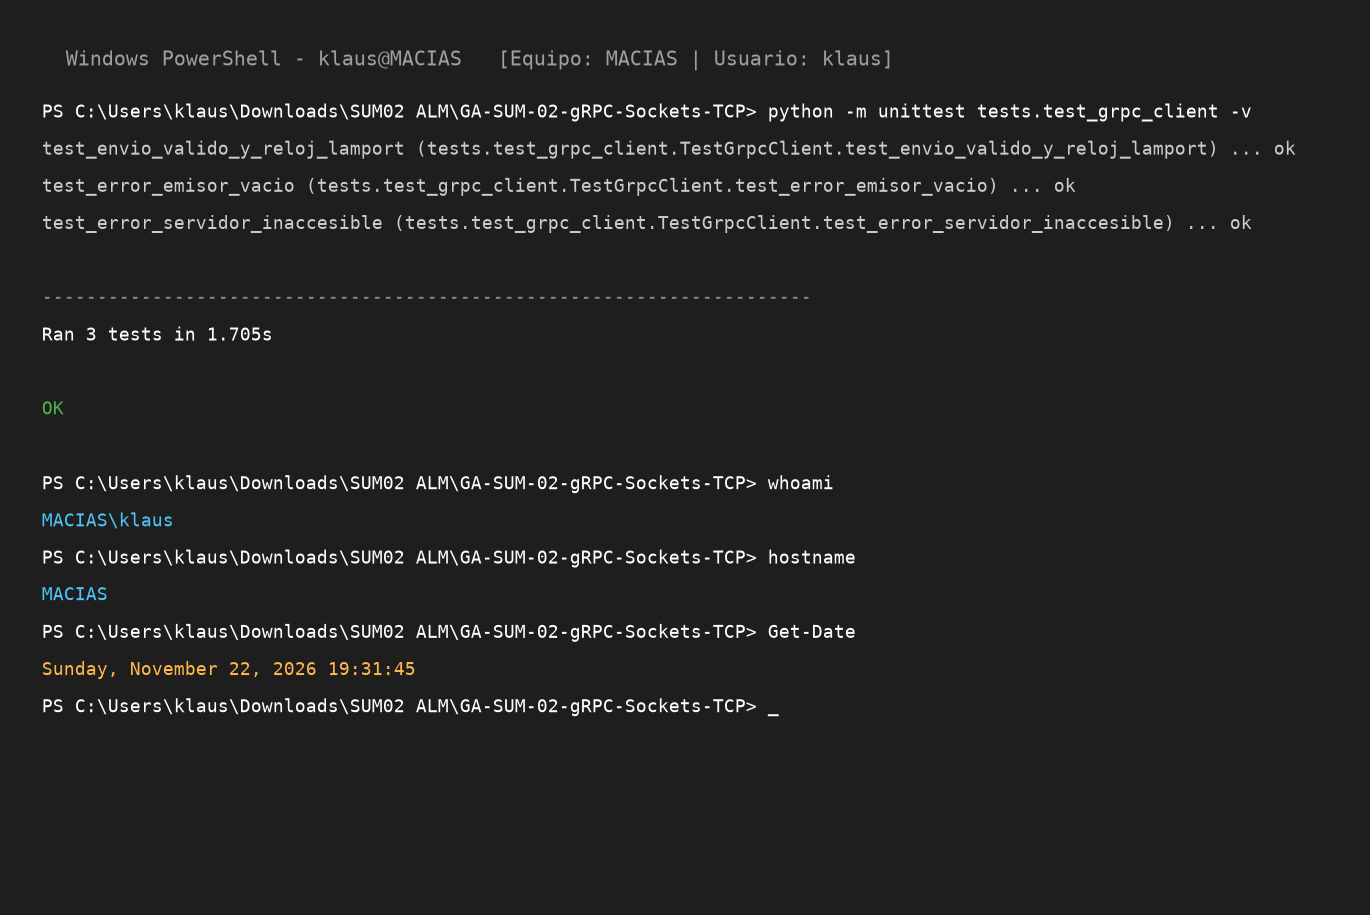
\includegraphics[width=\linewidth]{informe/capturas/captura_pruebas_cliente_cesar.png}
  \caption{Ejecución de las pruebas unitarias del cliente gRPC superadas satisfactoriamente (César Macías).}
  \label{fig:pruebas_cliente_cesar}
\end{figure}

\begin{figure}[htbp]
  \centering
  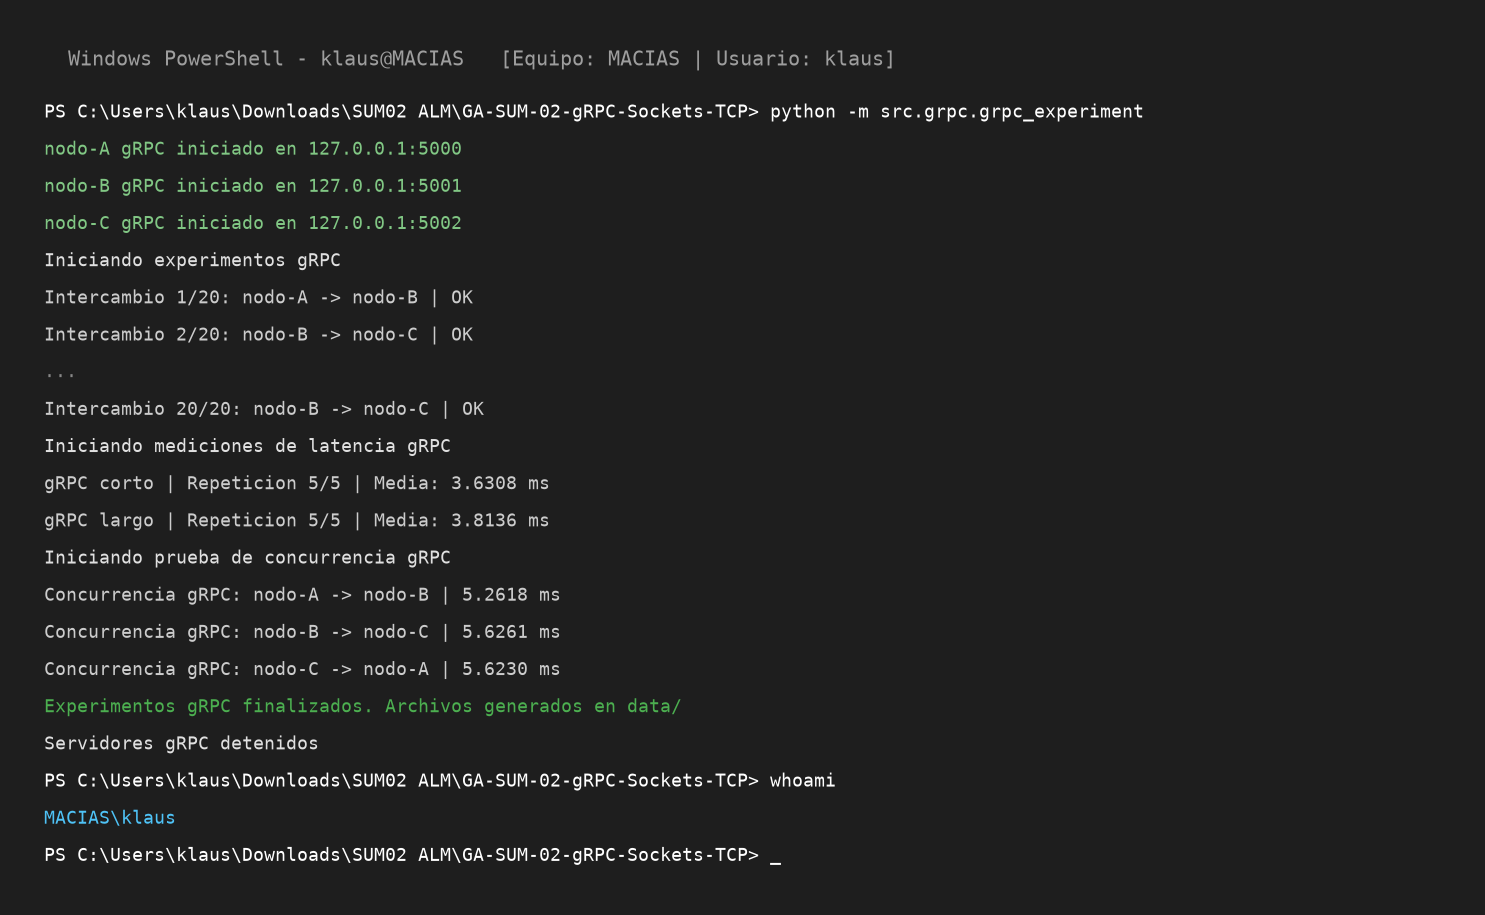
\includegraphics[width=\linewidth]{informe/capturas/captura_experimento_grpc_cesar.png}
  \caption{Ejecución completa del script de experimentación gRPC en el entorno local (César Macías).}
  \label{fig:experimento_grpc_cesar}
\end{figure}

\subsection{Conclusión individual: César Macías}

Mi responsabilidad en este proyecto abarcó el desarrollo del cliente gRPC
(\texttt{src/grpc/grpc\_client.py}), la ejecución y automatización de la batería
de experimentos distribuidos (\texttt{src/grpc/grpc\_experiment.py}) y la
implementación de las pruebas unitarias correspondientes en
\texttt{tests/test\_grpc\_client.py}.

La sincronización de los relojes lógicos de Lamport demostró ser fundamental para
mantener la consistencia temporal en un entorno asíncrono y distribuido. Implementar
la actualización del reloj antes de emitir la llamada y tras la llegada del acuse
permitió constatar que la relación de precedencia causal se cumple con exactitud en
todas las corridas, tanto en los intercambios secuenciales como bajo condiciones
concurrentes. Asimismo, la serialización binaria con Protocol Buffers redujo la
complejidad del cliente respecto a TCP, al delegar la codificación de tipos y
ofrecer stubs tipados que validan la interfaz antes del tránsito por la red.

Las pruebas unitarias implementadas verificaron no solo el caso nominal, sino
también la robustez ante destinos caídos y validaciones de argumentos. Con estas
adiciones, la suite de pruebas del proyecto alcanzó 56 pruebas unitarias exitosas,
garantizando la fiabilidad de las mediciones y la base de datos experimental
utilizada para la comparación estadística entre ambos paradigmas.


\section{Análisis comparativo entre TCP y gRPC}
\label{sec:comparacion-tcp-grpc}

Una vez implementados los mecanismos de comunicación mediante sockets TCP y
gRPC, se realizó un análisis comparativo para observar cómo se comportan
ambos cuando intercambian mensajes entre los tres nodos del sistema. Para
ello, se utilizaron los resultados obtenidos durante los experimentos,
considerando principalmente la latencia, el throughput y las solicitudes
concurrentes.

El propósito de esta comparación es identificar las diferencias observadas
entre las dos implementaciones bajo las condiciones de prueba utilizadas,
sin asumir que los resultados necesariamente serán iguales en otros equipos
o entornos de red.

\subsection{Metodología del análisis comparativo}

Ambos mecanismos se midieron en el mismo equipo, sobre \texttt{localhost},
con tres nodos, los mismos tamaños de carga útil (100 y 10.240 bytes), cinco
repeticiones de cien muestras por tamaño y una prueba de tres solicitudes
concurrentes. Estas condiciones permiten comparar las corridas registradas,
aunque no eliminan toda variación temporal del equipo.

Para realizar la comparación se utilizaron los archivos
\texttt{data/tcp\_latency.csv} y \texttt{data/grpc\_latency.csv}, que
contienen las mediciones obtenidas con cada mecanismo.

Se trabajó con dos tamaños de mensaje: uno corto de 100 bytes y otro largo
de 10.240 bytes. Para cada combinación se realizaron cinco repeticiones
de cien muestras, por lo que se obtuvieron 500 mediciones para TCP y
otras 500 para gRPC en cada tamaño.

En total, se analizaron 2.000 registros de latencia. A partir de estos
datos se calcularon la media, mediana, mínimo, máximo, desviación estándar,
percentil 95 (P95) y throughput promedio.

También se calcularon intervalos de confianza estimados del 95\,\% para
las medias y para las diferencias observadas entre los mecanismos. Estos
valores permiten apreciar la variabilidad de las mediciones, aunque su
interpretación debe considerar que las muestras proceden de repeticiones
de una misma configuración experimental.

El procesamiento se realizó mediante el módulo
\texttt{analysis/compare\_tcp\_grpc.py}, que genera los archivos CSV y
los gráficos utilizados en esta sección.

\subsection{Comparación de latencia}

La latencia representa el tiempo que tarda una comunicación en completar
el intercambio de solicitud y respuesta. Esta métrica permite observar
cuánto tiempo necesita cada mecanismo para realizar una comunicación
bajo las condiciones de las pruebas.

En la Tabla~\ref{tab:comparacion-latencia} se presentan los resultados
obtenidos para los dos tamaños de mensaje.

\begin{table}[htbp]
\centering
\caption{Comparación estadística de latencia entre TCP y gRPC}
\label{tab:comparacion-latencia}
\begin{tabular}{llrrr}
\hline
\textbf{Tamaño} & \textbf{Mecanismo} &
\textbf{Muestras} & \textbf{Media (ms)} &
\textbf{P95 (ms)} \\
\hline
Corto & TCP  & 500 & 7,220525 & 13,501700 \\
Corto & gRPC & 500 & 3,634639 & 5,048150 \\
Largo & TCP  & 500 & 4,850986 & 7,165695 \\
Largo & gRPC & 500 & 3,271925 & 5,009995 \\
\hline
\end{tabular}
\end{table}

Los resultados muestran que gRPC registró una latencia media menor en
ambos tamaños de mensaje. Para los mensajes cortos, la diferencia fue
de aproximadamente 3,59 ms, mientras que para los mensajes largos fue
de 1,58 ms.

En términos porcentuales, la reducción observada de latencia con gRPC
fue del 49,66\,\% para los mensajes cortos y del 32,55\,\% para los
largos, tomando como referencia los valores medios de TCP.

Un detalle que también llama la atención es que, en esta ejecución,
los mensajes largos presentaron una latencia media menor que los cortos
en ambos mecanismos. Esto demuestra que el tamaño del mensaje no fue
el único factor que intervino en los tiempos registrados.


\begin{table}[htbp]
\centering
\caption{Intervalos de confianza estimados de las diferencias de latencia}
\label{tab:intervalos-confianza}
\begin{tabular}{lrr}
\hline
\textbf{Tamaño} & \textbf{Límite inferior (ms)} &
\textbf{Límite superior (ms)} \\
\hline
Corto & 3,226532 & 3,945241 \\
Largo & 1,244700 & 1,913422 \\
\hline
\end{tabular}
\end{table}

Los intervalos estimados muestran que, en las dos categorías,
la diferencia media observada favoreció a gRPC. Estos valores
deben interpretarse considerando los supuestos estadísticos
del cálculo y la posible dependencia entre las mediciones
de una misma corrida.


\subsection{Comparación del throughput}

Además de la latencia, se comparó el throughput promedio, que representa
la cantidad de mensajes procesados por segundo según las mediciones
registradas durante los experimentos.

\begin{table}[htbp]
\centering
\caption{Throughput promedio por mecanismo y tamaño de mensaje}
\label{tab:comparacion-throughput}
\begin{tabular}{lrrr}
\hline
\textbf{Tamaño} & \textbf{TCP (msg/s)} &
\textbf{gRPC (msg/s)} & \textbf{Variación (\%)} \\
\hline
Corto & 144,301253 & 275,372357 & 90,83 \\
Largo & 204,265171 & 306,316840 & 49,96 \\
\hline
\end{tabular}
\end{table}

En los dos tamaños de mensaje, gRPC obtuvo un throughput promedio
superior al registrado con TCP. La diferencia fue más amplia para
los mensajes cortos, donde el valor de gRPC fue aproximadamente un
90,83\,\% mayor.

Para los mensajes largos también se observó una diferencia favorable
a gRPC, con un incremento del 49,96\,\%.

Estos resultados muestran que, durante las corridas realizadas,
gRPC procesó una mayor cantidad de mensajes por segundo según la
métrica utilizada. Sin embargo, este comportamiento corresponde
a la configuración experimental evaluada y no debe considerarse
una ventaja garantizada en cualquier escenario.

\subsection{Comportamiento ante solicitudes concurrentes}

También se compararon los resultados de las pruebas de concurrencia.
En esta parte se realizaron tres comunicaciones simultáneas entre
los nodos A, B y C, registrando el tiempo de respuesta de cada una.

\begin{table}[htbp]
\centering
\caption{Resultados de las pruebas de concurrencia}
\label{tab:comparacion-concurrencia}
\begin{tabular}{lrrr}
\hline
\textbf{Métrica} & \textbf{TCP} & \textbf{gRPC} &
\textbf{Unidad} \\
\hline
Solicitudes & 3 & 3 & -- \\
Respuestas exitosas & 3 & 3 & -- \\
Latencia media & 6,335300 & 13,068033 & ms \\
Latencia mínima & 6,115400 & 12,071400 & ms \\
Latencia máxima & 6,678700 & 13,938400 & ms \\
Desviación estándar & 0,301274 & 0,939883 & ms \\
\hline
\end{tabular}
\end{table}

A diferencia de los resultados de latencia individual, en esta prueba
TCP presentó un tiempo medio de respuesta menor que gRPC. Los tres
mecanismos de comunicación completaron correctamente sus solicitudes,
por lo que ambas implementaciones respondieron ante las comunicaciones
simultáneas realizadas.

Este resultado es importante porque permite observar que el
comportamiento de los mecanismos puede cambiar según el tipo de prueba.
Aunque gRPC obtuvo mejores valores en las mediciones de latencia y
throughput, TCP registró menor tiempo de respuesta en esta prueba
concurrente.

De todas formas, se debe considerar que solamente se utilizaron tres
solicitudes. Por esta razón, no sería correcto afirmar que TCP tiene
mejor escalabilidad a partir de estos resultados.

\subsection{Visualización de los resultados}

El gráfico de barras de latencia incluye intervalos de confianza estimados
del 95\,\% para las medias de cada grupo.

\begin{figure}[htbp]
\centering
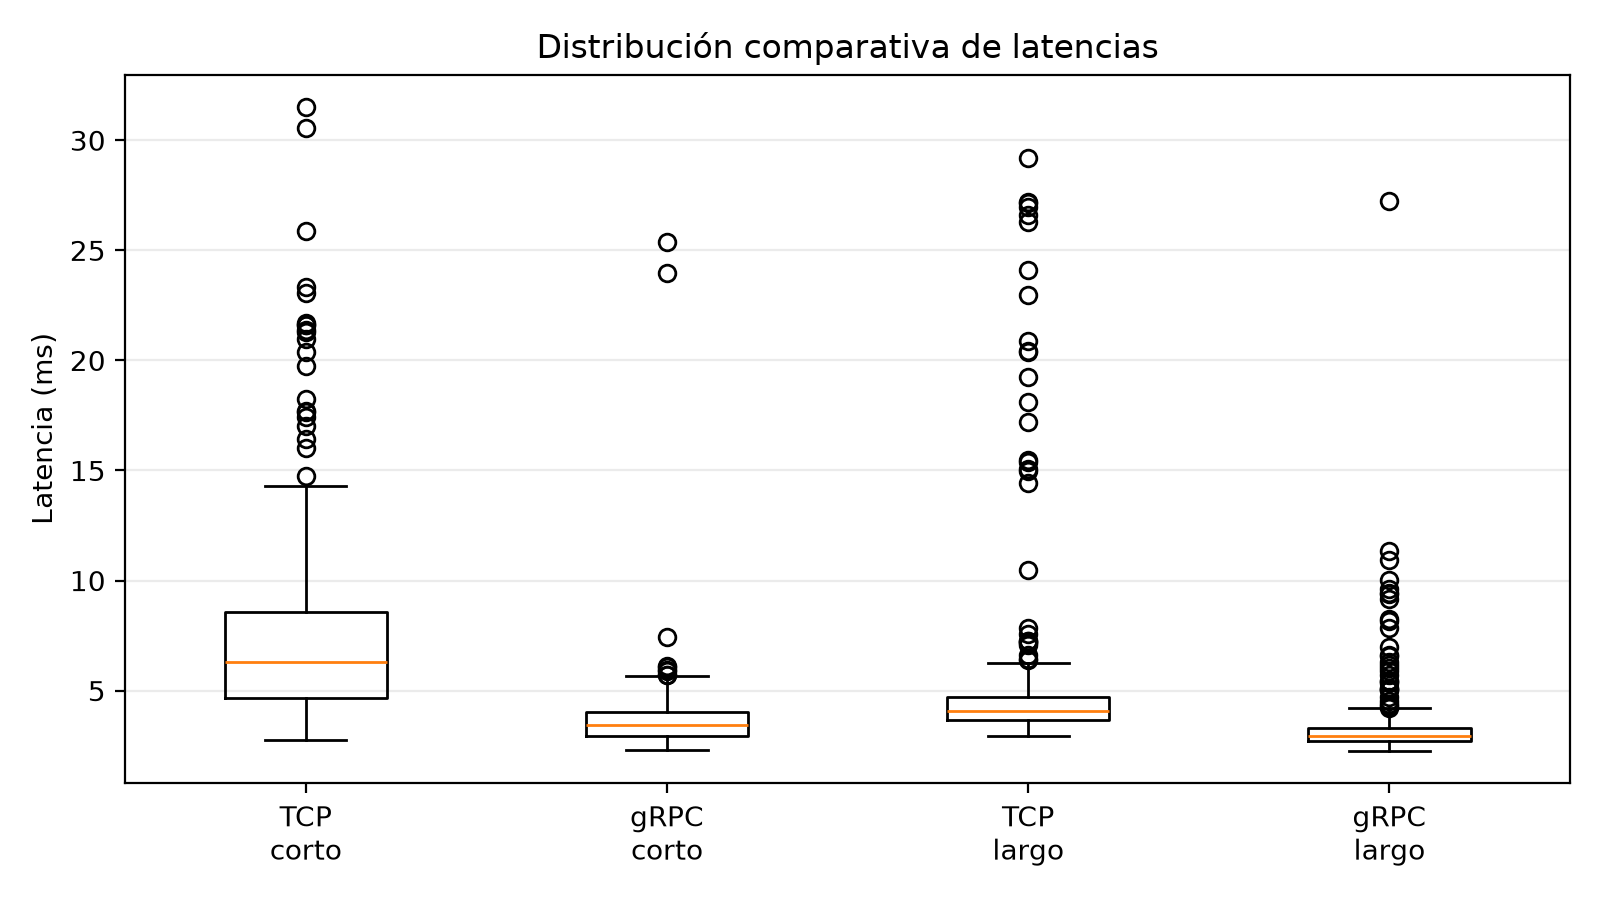
\includegraphics[width=0.85\linewidth]{analysis/figures/comparative_boxplot.png}
\caption{Diagramas de caja de las latencias TCP y gRPC por tamaño de mensaje.}
\label{fig:comparative-boxplot}
\end{figure}

Para facilitar la interpretación de los datos, el programa de análisis
generó tres gráficos que permiten observar las diferencias entre TCP
y gRPC.

\begin{figure}[htbp]
\centering
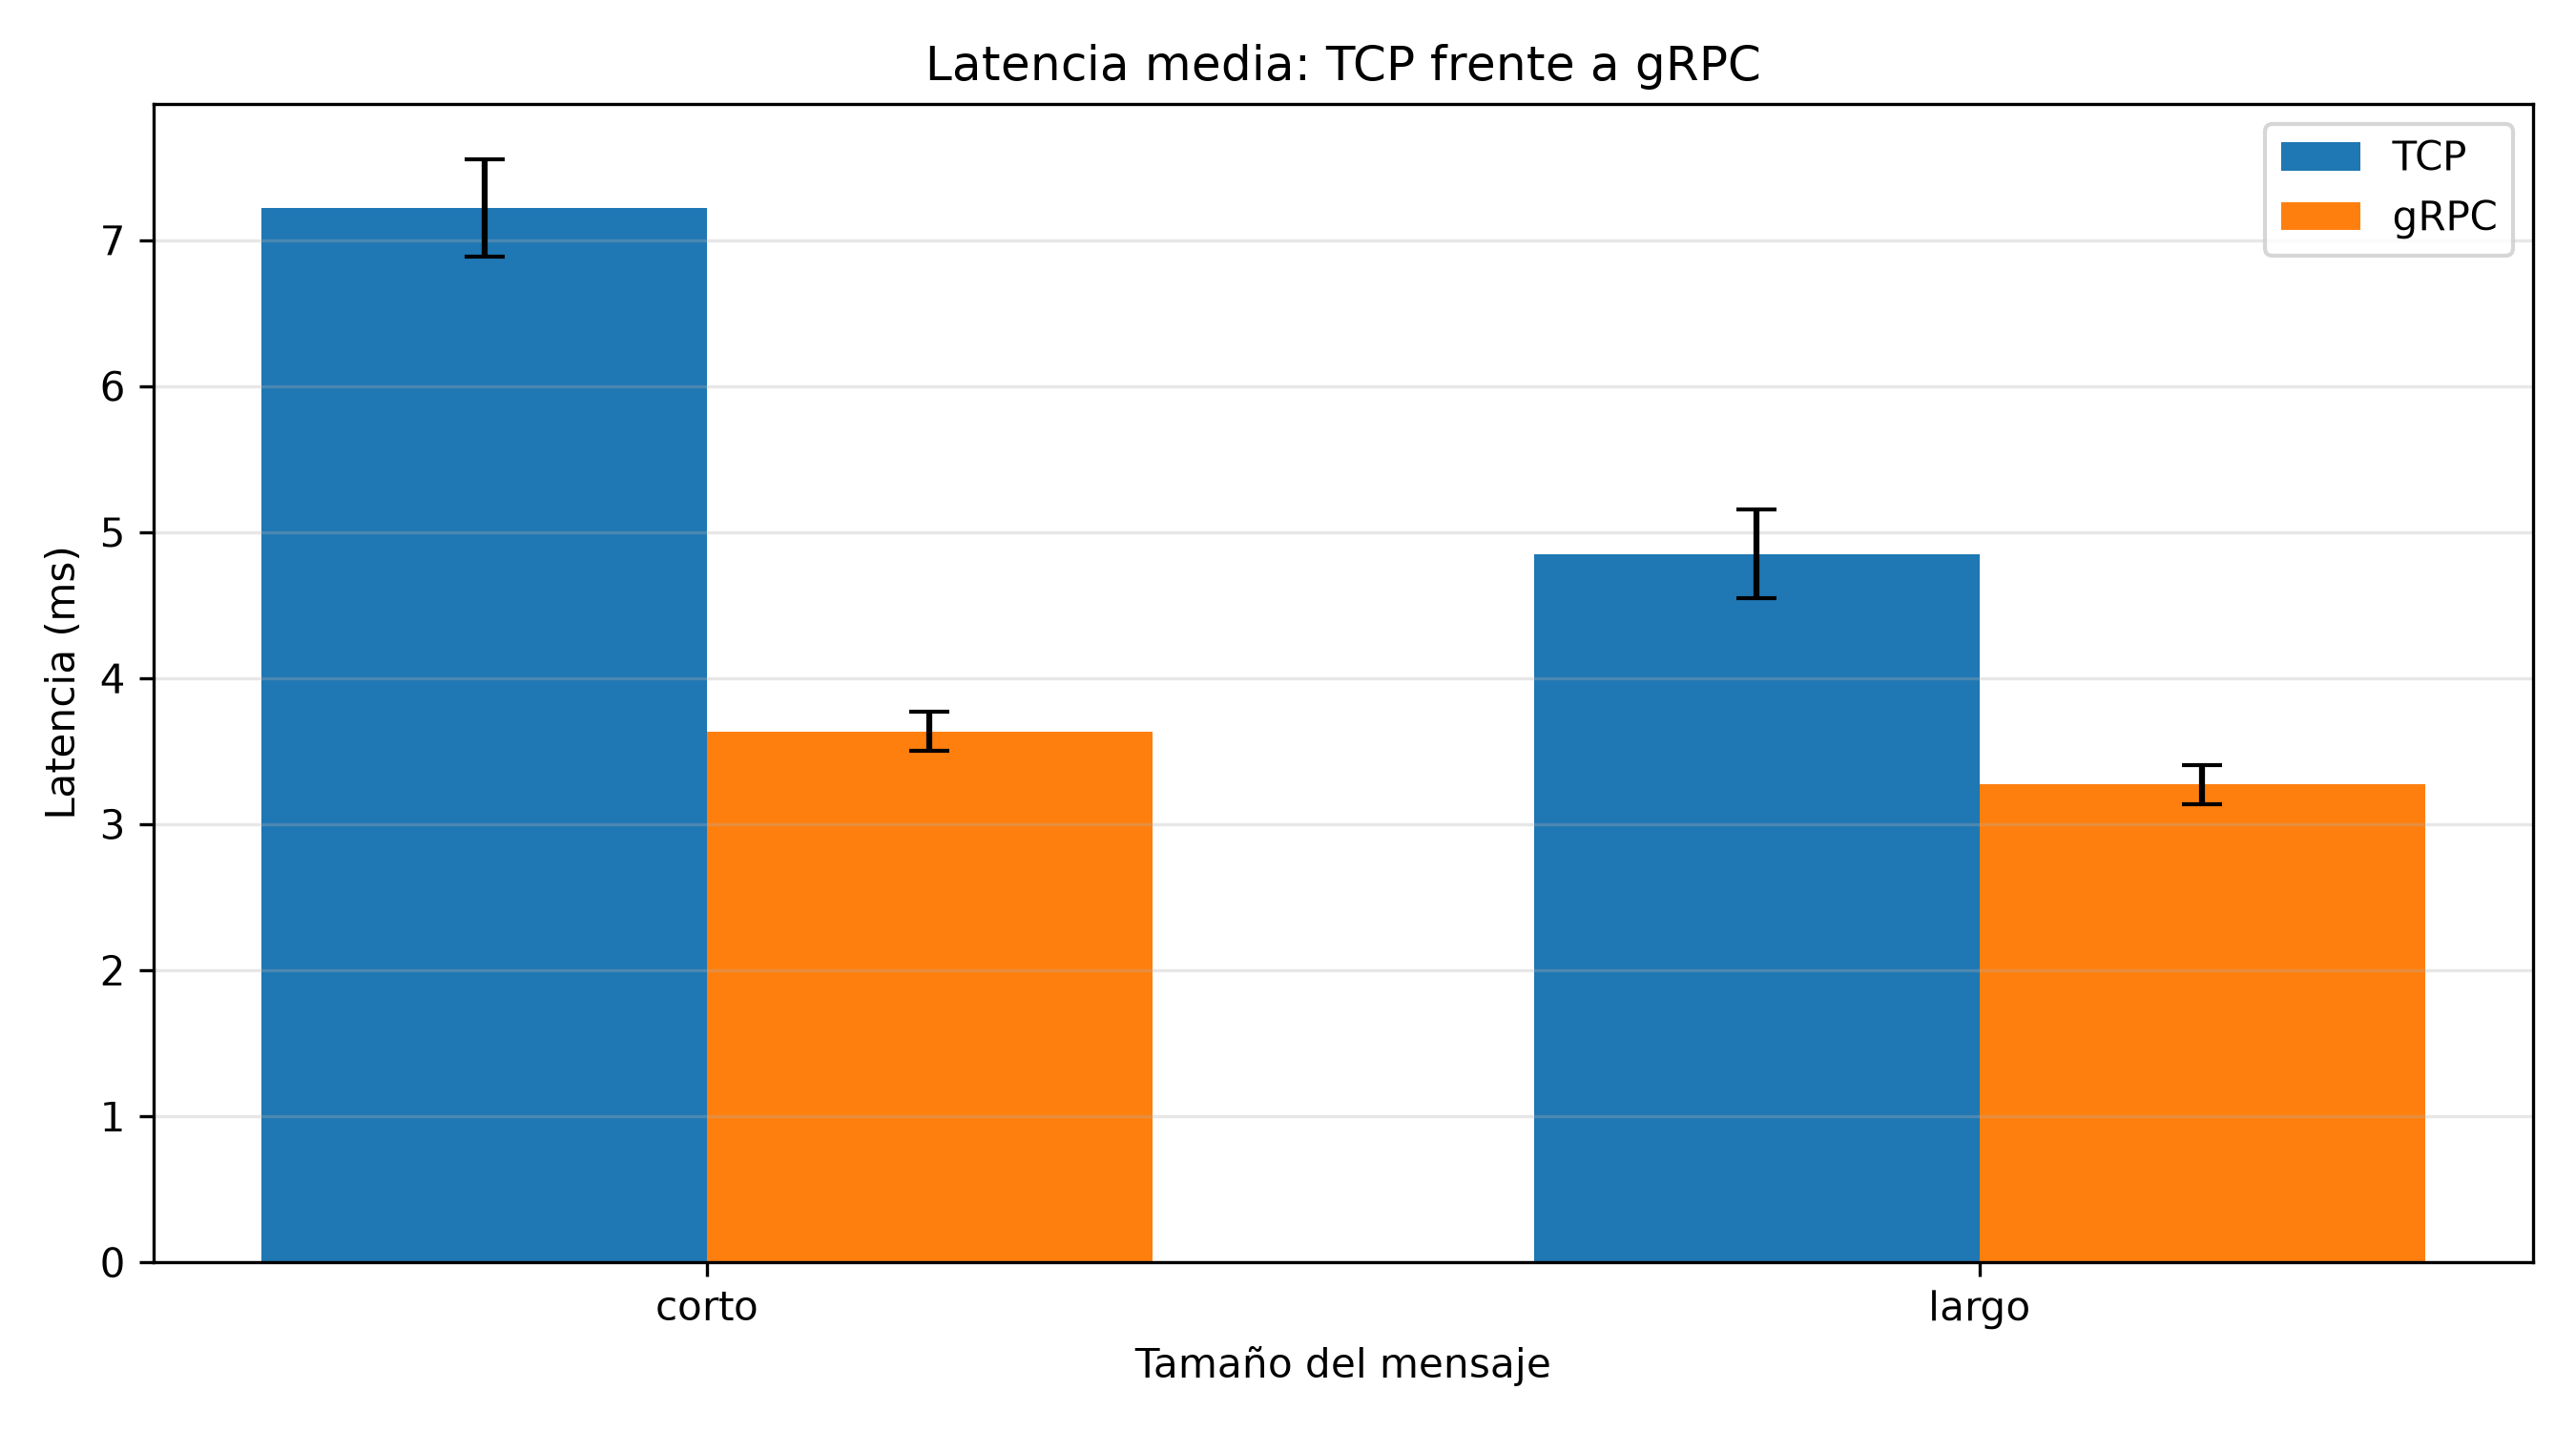
\includegraphics[width=0.85\linewidth]
{analysis/figures/comparative_latency.png}
\caption{Comparación de latencia entre TCP y gRPC.}
\label{fig:comparative-latency}
\end{figure}

La Figura~\ref{fig:comparative-latency} permite observar las diferencias
entre las latencias medias de ambos mecanismos para los dos tamaños
de mensaje. En esta ejecución, gRPC presentó valores inferiores en
ambos casos.

\begin{figure}[htbp]
\centering
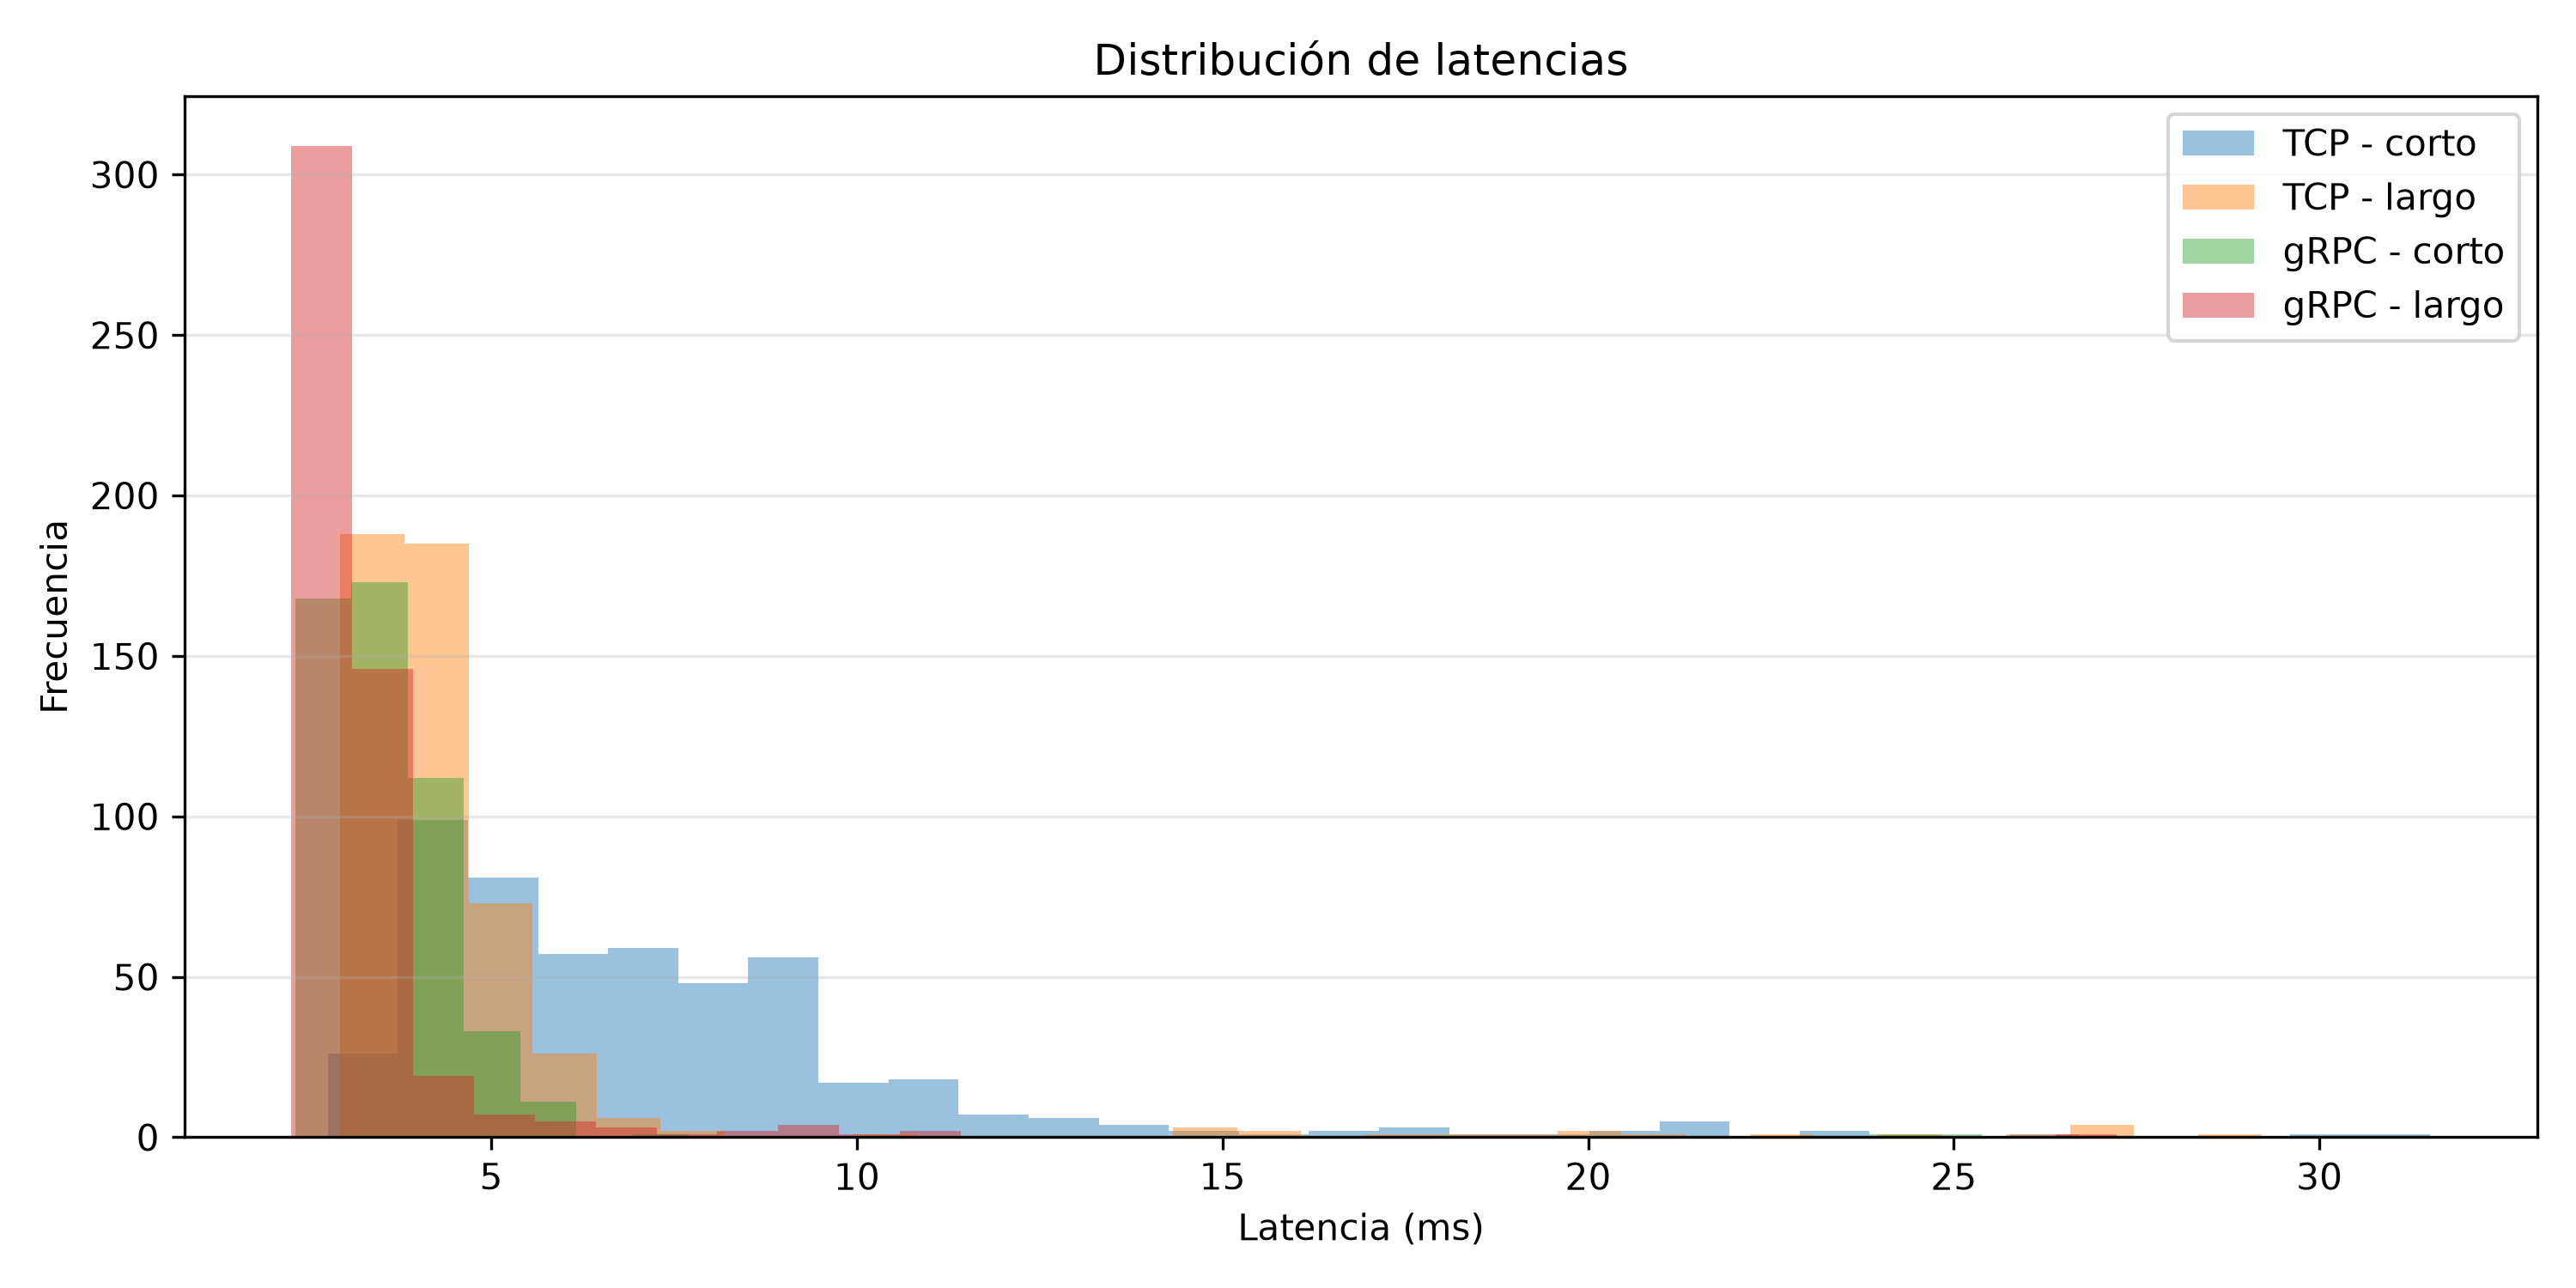
\includegraphics[width=0.85\linewidth]
{analysis/figures/comparative_distribution.png}
\caption{Distribución de las latencias registradas.}
\label{fig:comparative-distribution}
\end{figure}

En la Figura~\ref{fig:comparative-distribution} se puede observar cómo
se distribuyeron las mediciones de latencia. Esta representación
complementa los valores medios, ya que permite apreciar la dispersión
de los tiempos registrados durante los experimentos.

\begin{figure}[htbp]
\centering
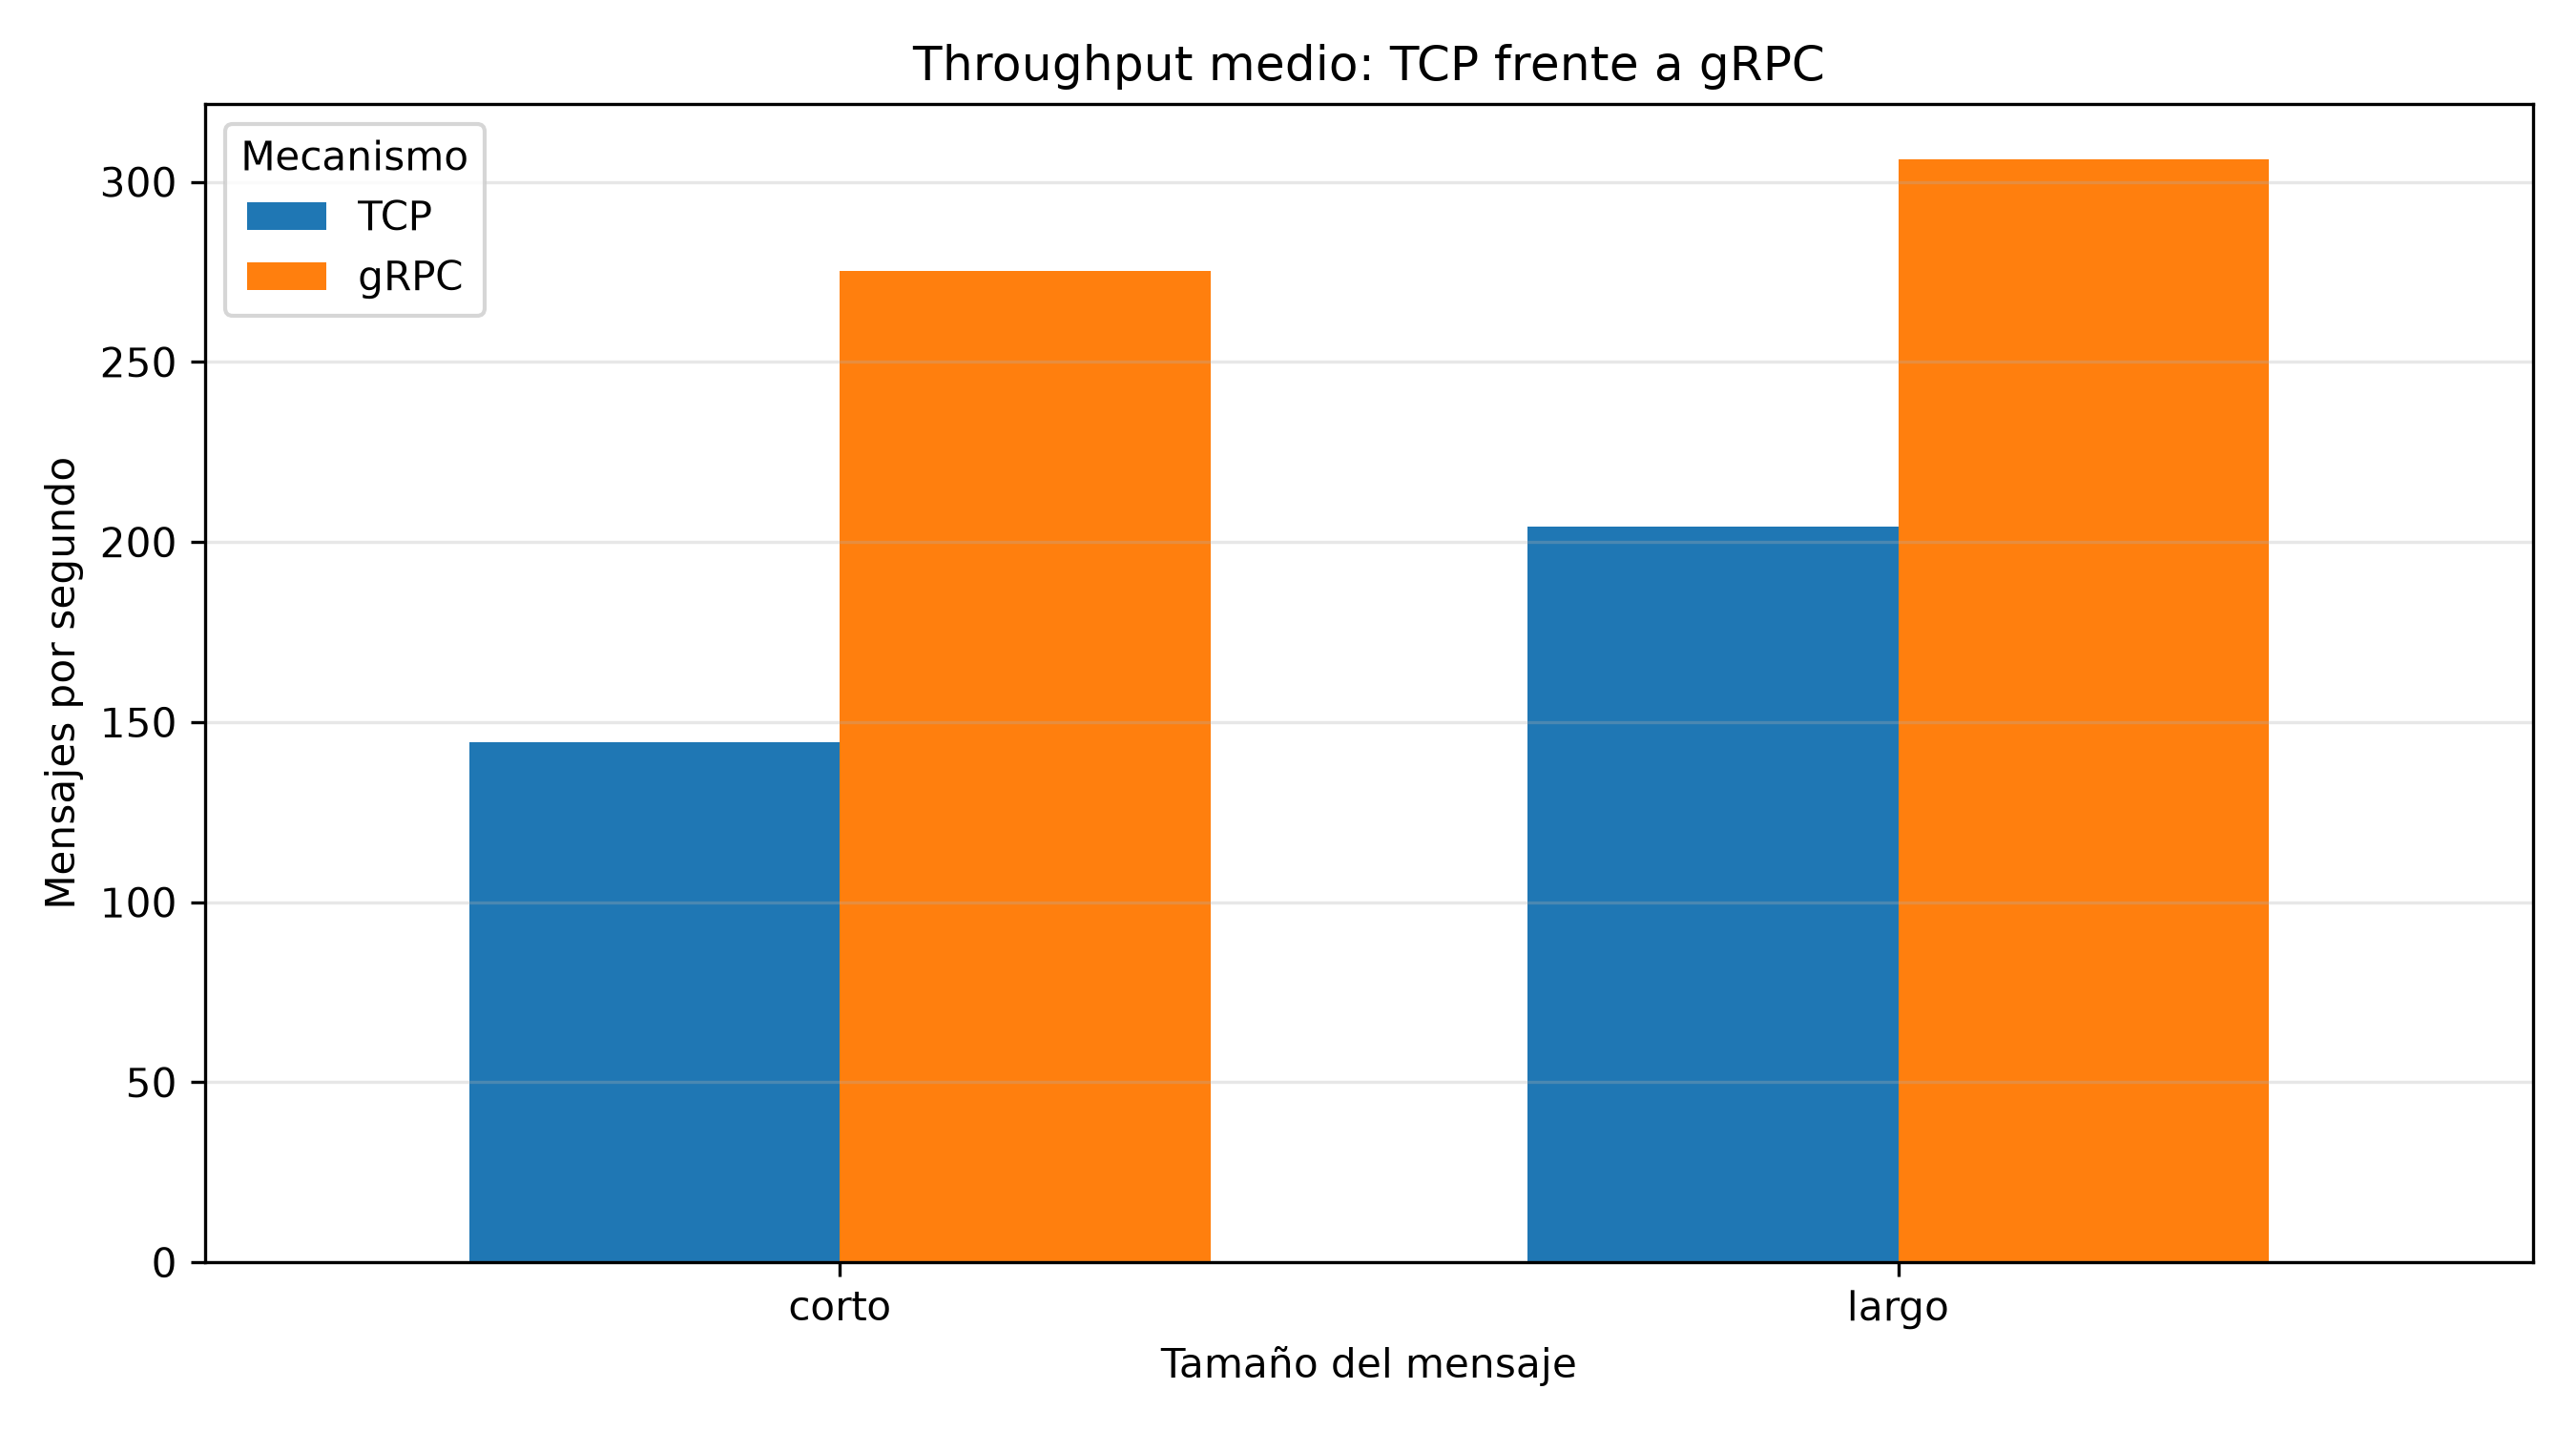
\includegraphics[width=0.85\linewidth]
{analysis/figures/comparative_throughput.png}
\caption{Comparación del throughput promedio.}
\label{fig:comparative-throughput}
\end{figure}

La Figura~\ref{fig:comparative-throughput} muestra que gRPC obtuvo
mayores valores de throughput para los dos tamaños de mensaje
evaluados, coincidiendo con los resultados de la tabla comparativa.

\subsection{Discusión y limitaciones}

Al revisar los resultados en conjunto, se observa que gRPC presentó
menor latencia media y mayor throughput en las pruebas individuales.
Por otro lado, TCP obtuvo menor latencia media en la prueba de tres
solicitudes concurrentes. Esto demuestra que no basta con utilizar
una sola métrica para determinar el comportamiento de un mecanismo
de comunicación.

También es necesario considerar las condiciones en las que se
realizaron los experimentos. Los tres nodos se ejecutaron en el mismo
equipo mediante la dirección local \texttt{127.0.0.1}, por lo que
no se evaluaron las variaciones propias de una red física entre
computadoras diferentes.

Además, las pruebas de concurrencia se limitaron a tres solicitudes
y no permiten determinar cómo responderían las implementaciones
ante una cantidad mayor de clientes.

Por estas razones, los resultados deben interpretarse como una
comparación de las dos implementaciones bajo las condiciones
específicas del proyecto. Para obtener conclusiones más amplias
sería necesario repetir las pruebas en diferentes entornos de red
y con distintos niveles de concurrencia.


\section{Conclusión individual: Jordan}

Durante mi participación en el proyecto me encargué de trabajar en la
verificación de los datos experimentales y en el análisis comparativo
entre TCP y gRPC. Esta parte me permitió comprender mejor cómo se
pueden evaluar dos mecanismos de comunicación a partir de mediciones
reales y no solamente de sus características teóricas.

Al revisar los resultados, observé que gRPC obtuvo una latencia media
menor y un throughput promedio mayor en las pruebas realizadas con
mensajes cortos y largos. Sin embargo, en la prueba de concurrencia
TCP registró un menor tiempo medio de respuesta. La reducción de la latencia
media de gRPC fue del 49,66\,\% en mensajes
cortos y del 32,55\,\% en mensajes largos frente a TCP. En la prueba de tres
solicitudes concurrentes, las medias fueron 6,335300~ms para TCP y
13,068033~ms para gRPC. Esto me permitió
entender que el rendimiento de un mecanismo no se puede valorar
utilizando una sola métrica, ya que su comportamiento puede variar
según las condiciones de ejecución.

También trabajé en la validación de los archivos CSV y en las pruebas
automatizadas para detectar datos incompletos, valores incorrectos
y resultados estadísticos inconsistentes. Comprobar que las pruebas
se ejecutaran correctamente fue importante para tener mayor confianza
en la información utilizada durante el análisis.

Una de las principales limitaciones que identifiqué fue que los tres
nodos se ejecutaron en el mismo equipo, utilizando la interfaz local.
Además, la prueba de concurrencia se limitó a tres solicitudes, por
lo que todavía sería necesario realizar experimentos adicionales
en diferentes equipos y con una mayor cantidad de comunicaciones.

En general, este trabajo me ayudó a relacionar los conceptos de
comunicación distribuida con su aplicación práctica. También aprendí
la importancia de validar los datos antes de interpretarlos y de
presentar conclusiones que realmente correspondan a los resultados
obtenidos.

\section{Conclusión individual: Washington Apunte}

Mi parte fue el contrato \texttt{servicio.proto} y el servidor gRPC. En el
contrato definí el servicio \texttt{ComunicacionNodos}, con la función
\texttt{EnviarMensaje}, y los mensajes \texttt{Mensaje} y \texttt{Acuse}. En el
servidor implementé esa función: valida la solicitud, actualiza el reloj de
Lamport, registra los eventos \texttt{receive} y \texttt{send} y devuelve el
acuse. Las llamadas se atienden con un grupo fijo de 10 hilos.

La decisión que más tuve que justificar fue usar \texttt{int64} para los tres
timestamps, aunque el reloj nunca es negativo. Lo elegí porque facilita la
compatibilidad con lenguajes sin enteros sin signo nativos y porque permite que
el servidor reciba un valor negativo y lo rechace con
\texttt{INVALID\_ARGUMENT}, como comprueba \texttt{test\_timestamp\_negativo}.

Escribí 6 pruebas para el servidor, que forman parte de las 56 del proyecto.
La de concurrencia lanza 30 llamadas desde 10 hilos y ningún timestamp se
repite, pero aprendí a no exagerar ese resultado: demuestra que los valores son
únicos, no que cada llamada sea atómica. También vi que el contrato fija los
tipos, pero no los valores: el emisor vacío y el timestamp negativo los sigue
validando mi servidor.

\section{Declaración de uso de inteligencia artificial}

\subsection{Washington Apunte}

Durante el desarrollo del proyecto, utilicé el modelo Claude Sonnet 5.5 únicamente como herramienta de apoyo y guía técnica. Su uso se limitó a la consulta de comandos de GitHub para navegar y gestionar el repositorio, la revisión ortográfica del documento y la estructuración de plantillas base en formato LaTeX para organizar los archivos del trabajo.

\subsection{César Macías}

En el desarrollo de mis actividades utilicé el modelo Gemini 3.8 como asistente de apoyo y consulta técnica. Su empleo se orientó al diseño y verificación de la estructura del cliente gRPC en Python, el manejo adecuado de excepciones \texttt{grpc.RpcError}, la formulación de casos de prueba unitaria con \texttt{unittest} para el cliente y la redacción clara de la documentación técnica y las secciones correspondientes en formato \LaTeX{}. Toda la lógica, la ejecución experimental y la validación de los datos fueron revisadas y verificadas directamente por el autor.

\subsection{Jordan Loor}

Durante el desarrollo del proyecto utilicé ChatGPT (GPT-6) como
herramienta de apoyo para resolver dudas puntuales sobre conceptos
de comunicación distribuida y análisis estadístico.
También lo utilicé como apoyo para mejorar la claridad y
organización de la documentación. La implementación, ejecución
de los experimentos y comprobación de los resultados estuvieron
a mi cargo.


\section{Aportes y trazabilidad}
\begin{table}[htbp]
\centering
\caption{Aportes identificados en el historial del repositorio}
\begin{tabular}{p{2.6cm}p{7.2cm}l}
\toprule
Integrante & Aporte & Commit \\
\midrule
Jordan Loor & Implementación y experimentación TCP & \href{https://github.com/jloors13/GA-SUM-02-gRPC-Sockets-TCP/commit/6ac87e5}{6ac87e5} \\
Washington Apunte & Contrato gRPC y pruebas del servidor & \href{https://github.com/jloors13/GA-SUM-02-gRPC-Sockets-TCP/commit/c2e9edc}{c2e9edc} \\
César Macías & Cliente gRPC y script experimental & \href{https://github.com/jloors13/GA-SUM-02-gRPC-Sockets-TCP/commit/9b30445}{9b30445} \\
\bottomrule
\end{tabular}
\end{table}

\printbibliography[heading=bibintoc,title={Referencias}]
\end{document}
